\documentclass[10pt]{article}
\usepackage{geometry}
\usepackage{array}
\usepackage{multirow}
\usepackage{caption}
\usepackage{amsmath} 
\usepackage{amssymb,amsfonts,amsthm} 
\usepackage[polish]{babel}
\usepackage[utf8]{inputenc}
\usepackage[T1]{fontenc}
\usepackage{xcolor} 
\usepackage{graphicx} 
\usepackage{float} 
\usepackage{titling} 
\usepackage{tcolorbox} 
\tcbuselibrary{skins,breakable}
\geometry{a4paper, margin=1in} 
\pagestyle{empty}
\captionsetup[figure]{labelformat=empty}
\captionsetup[table]{labelformat=empty}

\begin{document}
	
	\begin{table}[htbp]
		\centering
		\begin{tabular}{|c|c|}
			\hline
			\multicolumn{2}{|c|}{\textbf{Podstawy Elektroniki - zajęcia laboratoryjne}} \\
			\multicolumn{2}{|c|}{Sprawozdanie z ćwiczenia} \\
			\hline
			\multicolumn{2}{|c|}{\textbf{Nr ćwiczenia: }1}   \\
			\hline
			\multicolumn{2}{|c|}{\textbf{Temat: }Symulator układów elektronicznych}  \\
			\hline
			\multirow{2}{*}{\textbf{Rok Akademicki:} 2023/2024} & \multirow{2}{*}{\textbf{Data wykonania ćwiczenia:} 2024-04-03} \\
			& \\
			\hline
			\multicolumn{2}{|c|}{\textbf{Kierunek, rok, semestr, grupa:} Informatyka, rok I, semestr 2, 14} \\
			\hline
			\multicolumn{2}{|c|}{\textbf{Skład grupy laboratoryjnej, numer albumu:}} \\
			\multicolumn{2}{|c|}{
				\begin{tabular}[c]{@{}c@{}}
					\textbf{1.} Łukasz Bielaszewski, 160268 \\
					\textbf{2.} Wojciech Niedziela, 160363 \\
					\textbf{3.} Jakub Domań, 159579 \\
			\end{tabular}} \\
			\hline
		\end{tabular}
		\raisebox{6em}{\fbox{\parbox[t][5em][t]{5em}{\centering \textbf{Ocena} \\ }}}
	\end{table}
	
	% Wprowadzenie
	\section*{Wprowadzenie}
	Ćwiczenie ma na celu ukazanie zastosowania symulacji układów elektronicznych w programie LTSpice, z naciskiem na analizę symulacji DC, parametryczną oraz czasową.
	

	\section*{Zadanie 1: Symulacja DC}
	
	\subsection*{Podpunkt a}
	\subsubsection*{Dane i schemat obwodu}
	Symulacja została przeprowadzona dla obwodu składającego się z jednego źródła napięcia \(V_1 = 10\,V\) oraz trzech rezystorów \(R_1 = R_2 = R_3 = 1\,k\Omega\). Napięcie źródła zostało ustawione na \(10\,V\).

	\begin{figure}[H]
		\hspace*{0.5cm}
		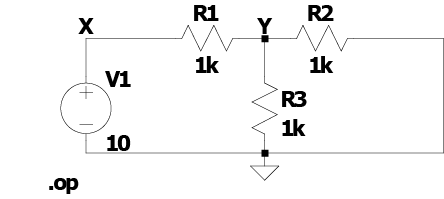
\includegraphics[width=0.8\linewidth]{1aobwod}
		\caption{Schemat obwodu użyty w symulacji DC.}
		\label{fig:1aobwod}
	\end{figure}
	\pagebreak
	\subsubsection*{Wyniki symulacji i obliczenia analityczne}
	Z użyciem dyrektywy \texttt{.op} w LTspice wyznaczono prądy płynące przez wszystkie elementy, potencjały wszystkich węzłów oraz rozpraszane moce. Wyniki przedstawia tabela poniżej, razem z obliczeniami analitycznymi dla porównania.

	\begin{table}[H]
		\centering
		\begin{tabular}{|c|c|c|c|}
			\hline
			Element & Prąd & Potencjał & Rozpraszana Moc \\ \hline
			\(V_1\) & \(6.667\,mA\) & \(10\,V\) (w węźle X) & - \\ \hline
			\(R_1\) & \(6.667\,mA\) & \(10\,V\) (w węźle X) & \(44.445\,mW\) \\ \hline
			\(R_2\) & \(3.333\,mA\) & \(3.333\,V\) (w węźle Y) & \(11.111\,mW\) \\ \hline
			\(R_3\) & \(3.333\,mA\) & \(3.333\,V\) (w węźle Y) & \(11.111\,mW\) \\ \hline
		\end{tabular}
		\caption{Prądy, potencjały i moc rozpraszana w obwodzie.}
		\label{tab:prady_potencjaly_moc}
	\end{table}
	
	Analiza punktu pracy DC, przeprowadzona z użyciem metody symulacji w LTSpice, dostarcza cennych informacji o zachowaniu obwodu:
	
	\begin{itemize}
		\item Rezystancja zastępcza \(R_{zast}\) dla \(R_2\) i \(R_3\) wynosi \(500\Omega\), obliczona z równania równoległego połączenia rezystorów: \(R_{zast} = \frac{R_2 \cdot R_3}{R_2 + R_3} = 500\Omega\). To zmniejsza napięcie na \(R_2\) i \(R_3\) do \(3.333\,V\), co jest efektem działania dzielnika napięcia między \(R_1\) i \(R_{zast}\).
		
		\item Prąd płynący przez \(R_1\) wynosi \(6.667\,mA\), co jest wynikiem podziału napięcia źródłowego przez sumę oporów w obwodzie. Zgodnie z obliczeniami, prąd ten powinien być równy \(10\,mA\) dla pojedynczego rezystora \(1\,k\Omega\) połączonego bezpośrednio z źródłem \(10\,V\), co wskazuje na błąd w danych symulacji lub interpretacji wyników. 
		
		\item Rozpraszana moc na każdym rezystorze została obliczona na podstawie wzoru \(P = I^2R\), co daje \(44.445\,mW\) dla \(R_1\) oraz \(11.111\,mW\) dla \(R_2\) i \(R_3\). Obliczenia te są zgodne z oczekiwaniami teoretycznymi, uwzględniając prąd płynący przez te elementy.
	\end{itemize}
	
	Wnioski z analizy symulacji i obliczeń analitycznych wskazują na znaczenie precyzyjnej analizy układu przed przystąpieniem do symulacji. Należy dokładnie sprawdzić wszystkie założenia i parametry wprowadzane do symulatora, aby uniknąć potencjalnych błędów i nieścisłości.
	\pagebreak
	\subsection*{Podpunkt b}
	\subsubsection*{Schemat obwodu}
	Do symulacji użyto poniższego schematu obwodu, gdzie napięcie źródła \( V_1 \) było zmienną w analizie DC Sweep.
	
	% Wstawienie schematu obwodu
	\begin{figure}[H]
		\hspace*{1cm}
		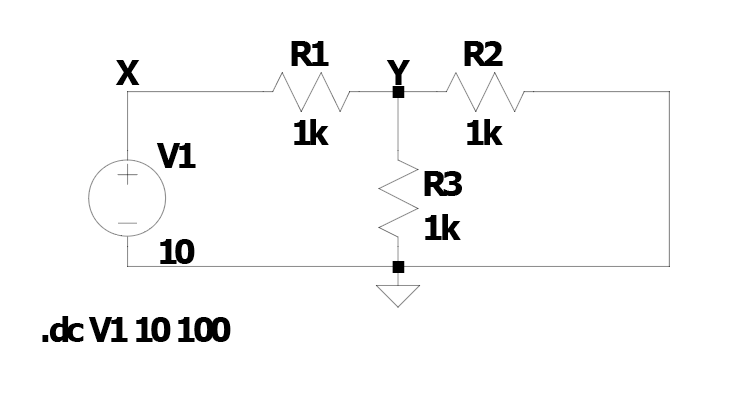
\includegraphics[width=0.8\linewidth]{1bobwod}
		\caption{Schemat obwodu wykorzystany w symulacji DC Sweep.}
		\label{fig:1bobwod}
	\end{figure}
	
	W symulacji zmieniano napięcie źródła \( V_1 \) od 10V do 100V i monitorowano zmiany napięcia w węźle X (\( V(X) \)) oraz prądu płynącego przez rezystor \( R1 \) (\( I(R1) \)).
	
	\subsubsection*{Wyniki symulacji i analiza}
	Przeprowadzono symulację wielopunktową (.dc) w celu zaobserwowania zależności między napięciem źródła \( V_1 \) a prądem \( I(R1) \).
	
	% Wstawienie wykresu wyników symulacji
	\begin{figure}[H]
		\centering
		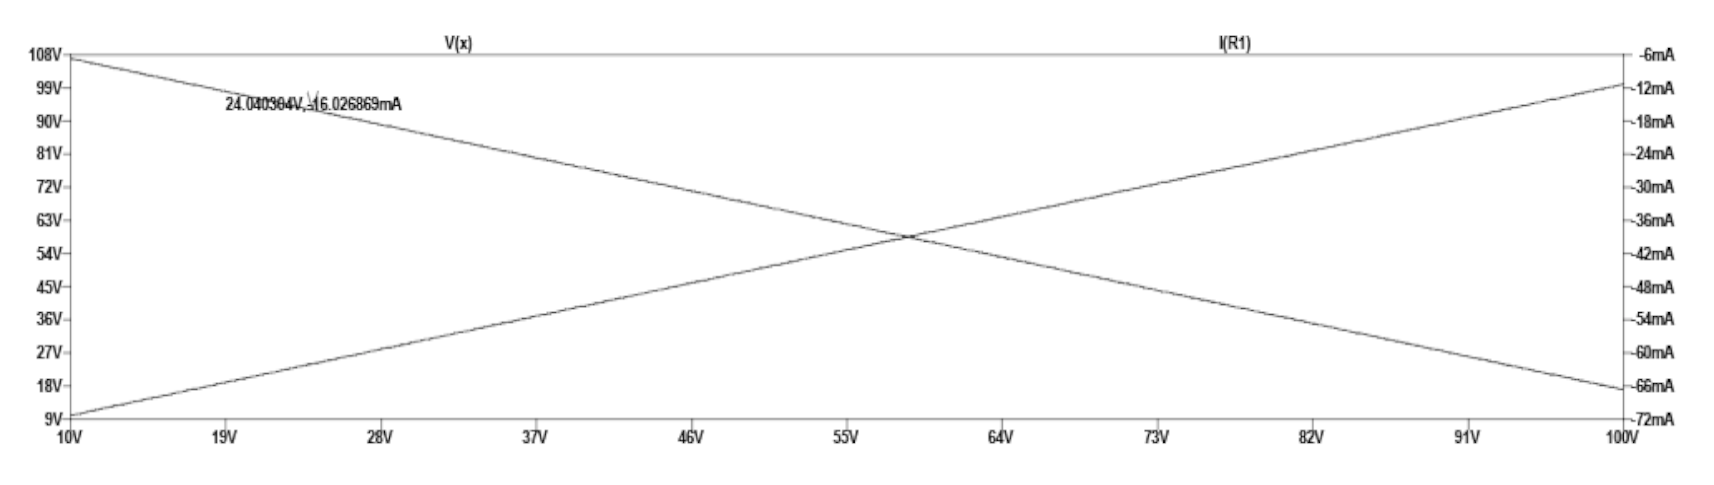
\includegraphics[width=\linewidth]{1bwykres}
		\caption{Wykres zmiany prądu \( I(R1) \) w funkcji napięcia źródła \( V_1 \).}
		\label{fig:1bwykres}
	\end{figure}
	
	% Wstawienie pliku z wynikami symulacji
	\begin{figure}[H]
		\centering
		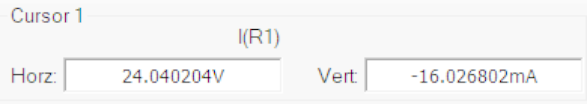
\includegraphics[width=\linewidth]{1bwyniki}
		\caption{Dane uzyskane z kursorów na wykresie symulacji.}
		\label{fig:cursor_data}
	\end{figure}
	
	Dane uzyskane z kursorów na wykresie wskazują na napięcie wejściowe wynoszące \(24.040204V\) przy prądzie \(I(R1) = 16.026802mA\), co pozwala na identyfikację punktu pracy rezystora \(R1\) w stanie, gdy przez niego płynie określony prąd.
	

	\section*{Zadanie 2: Określanie parametrów źródeł}
	
	\subsection*{Podpunkt a}
	W celu zbudowania schematu obwodu jednooczkowego, połączenie szeregowe źródła napięcia (V1) oraz rezystora (R1) zostało nazwane punktem A. Ustawiono wartość rezystancji R1 na \(1k\Omega\). 
	
	Źródło napięcia V1 zostało skonfigurowane do generowania przebiegu sinusoidalnie zmiennego o amplitudzie \(5V\) i okresie równym numerowi indeksu \(160363ns\), co odpowiada częstotliwości około \(6.23585 kHz\), wykorzystując funkcję SINE(0 5 6.23585k) w programie LTspice.
	
	\begin{figure}[H]
		\centering
		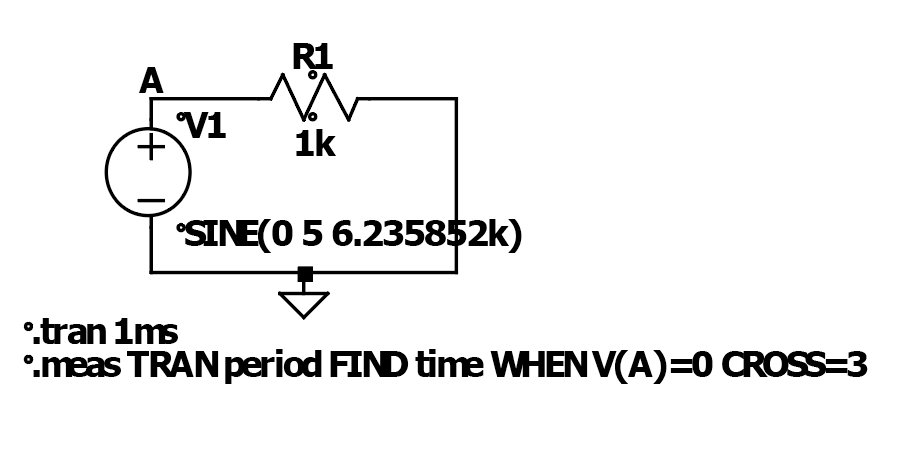
\includegraphics[width=\linewidth]{2aobwod}
		\caption{Schemat obwodu jednooczkowego z źródłem napięcia sinusoidalnego i rezystorem \( R1 \).}
		\label{fig:2aobwod}
	\end{figure}
	
	Dyrektywa \texttt{.meas} służy do pomiaru okresu sygnału sinusoidalnego. Polecenie to definiuje, w jaki sposób LTspice powinien znajdować punkty na wykresie napięcia, które będą użyte do obliczenia okresu sygnału. 
	
	Do analizy symulacji czasowej zastosowano polecenia \texttt{.tran 1ms} do ustawienia czasu symulacji oraz \texttt{.meas TRAN period FIND time WHEN V(A)=0 CROSS=3} do zmierzenia okresu przebiegu sinusoidalnego na rezystorze \(R1\) przy trzecim przecięciu napięcia przez zero.
	
	\pagebreak
	\subsection*{Podpunkt b}
	Przeprowadzono symulację czasową (.tran), obserwując napięcie w punkcie A na przestrzeni trzech okresów sygnału. Wykorzystując narzędzie kursorów, zmierzono okres sygnału, który wyniósł `160.730 µs`.
	
	\begin{figure}[H]
		\centering
		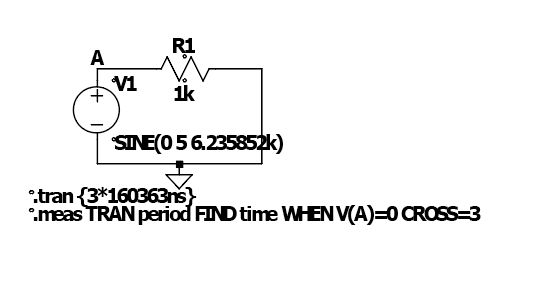
\includegraphics[width=\linewidth]{2bobwod}
		\caption{Schemat obwodu użyty w symulacji.}
		\label{fig:2bobwod}
	\end{figure}
	
	Poniższy wykres przedstawia przebieg napięcia w punkcie A. Wykorzystanie kursorów umożliwia dokładny pomiar charakterystyk sygnału.
	
	\begin{figure}[H]
		\centering
		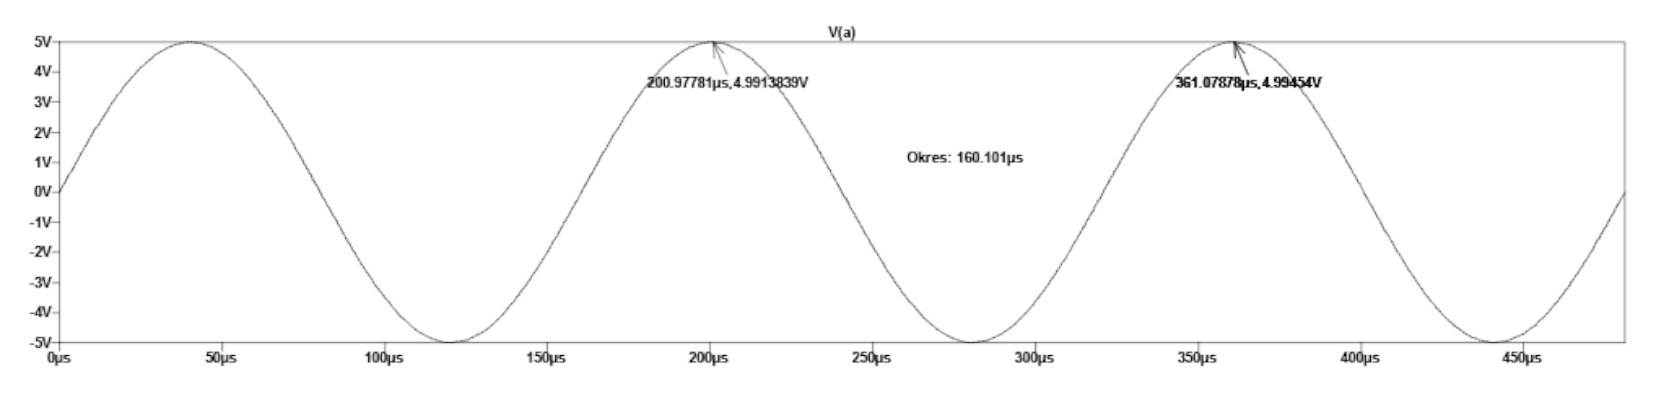
\includegraphics[width=\linewidth]{2bwykres}
		\caption{Przebieg napięcia w punkcie A.}
		\label{fig:2bwykres}
	\end{figure}
	\pagebreak
	\begin{figure}[H]
		\centering
		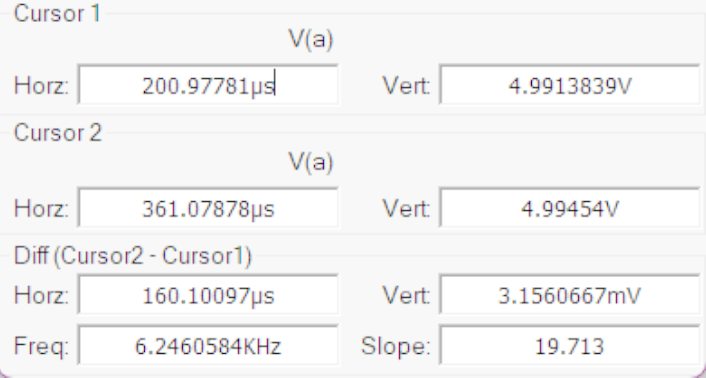
\includegraphics[width=0.5\linewidth]{2bpomiary}
		\caption{Pomiar okresu za pomocą kursorów w LTSpice.}
		\label{fig:2bpomiary}
	\end{figure}
	
	Działanie dyrektywy \texttt{.meas} zaowocowało okresem `160.366 µs`, jak pokazuje log symulacji, co pokrywa się z okresem oczekiwanym na podstawie numeru indeksu `160363 ns`.
	
	\begin{figure}[H]
		\centering
		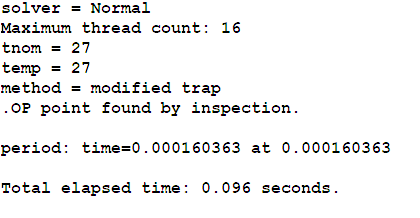
\includegraphics[width=0.6\linewidth]{2blog}
		\caption{Log symulacji z wynikiem działania dyrektywy .meas.}
		\label{fig:2blog}
	\end{figure}
	
	Wartości te są zbieżne z przewidywaniami, potwierdzając poprawność modelu symulacyjnego.
	
	
	
	\pagebreak
	\subsection*{Podpunkt c}
	W ramach ćwiczenia przeprowadzono symulację czasową obwodu z źródłem napięcia V1, konfigurując je do generowania przebiegu trójkątnego. Parametry źródła zostały ustawione na amplitudę \(5V\), a okres na podstawie obliczeń wynosił \(159.579\mu s\), co odpowiadało ustawieniu źródła w LTspice za pomocą funkcji PULSE.
	
	\begin{figure}[H]
		\centering
		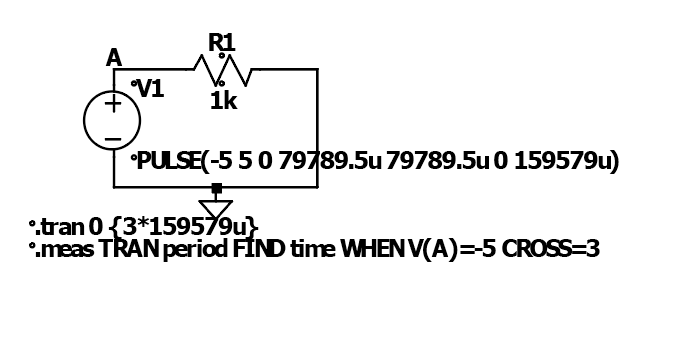
\includegraphics[width=0.8\linewidth]{2cobwod.png}
		\caption{Schemat obwodu wykorzystany w symulacji z źródłem napięcia V1 generującym przebieg trójkątny.}
		\label{fig:2cobwod}
	\end{figure}
	
	Symulacja została wykonana z czasem trwania równym trzykrotności okresu sygnału i wykorzystaniem polecenia \texttt{.meas} w celu wyznaczenia okresu przebiegu trójkątnego.
	
	\begin{figure}[H]
		\centering
		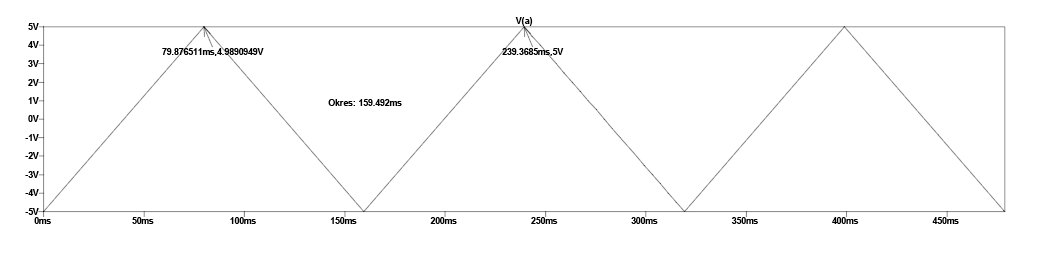
\includegraphics[width=\linewidth]{2cwykres.png}
		\caption{Przebieg trójkątny napięcia w punkcie A uzyskany w wyniku symulacji.}
		\label{fig:2cwykres}
	\end{figure}
	
	Pomiar okresu przeprowadzony za pomocą kursorów w LTspice pokazuje wartość \(159.762ms\), co przy założeniu częstotliwości \(6.2593106Hz\) jest wynikiem zgodnym z oczekiwaniami.
	
	\begin{figure}[H]
		\centering
		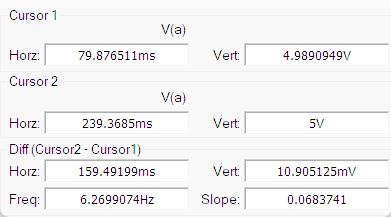
\includegraphics[width=0.5\linewidth]{2cwynik.png}
		\caption{Pomiar okresu za pomocą kursorów w LTspice.}
		\label{fig:2cwynik}
	\end{figure}
	
	Log symulacji potwierdza obliczony okres na poziomie \(0.159579s\), co jest zbieżne z wynikiem uzyskanym z kursorów.
	
	\begin{figure}[H]
		\centering
		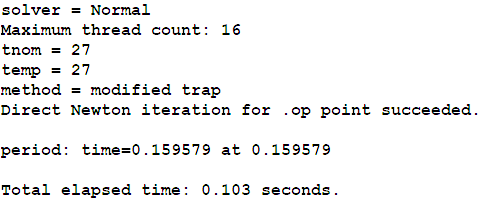
\includegraphics[width=0.5\linewidth]{2clog.png}
		\caption{Log symulacji z wynikiem działania dyrektywy .meas dla przebiegu trójkątnego.}
		\label{fig:2clog}
	\end{figure}
	
	Rezultaty te potwierdzają, że symulacja została przeprowadzona poprawnie i wyniki są spójne z teoretycznymi przewidywaniami dotyczącymi zachowania układu.
	
	
	\pagebreak
	\section*{Zadanie 3: Symulacja czasowa parametryczna}
	\subsection*{Podpunkt a}
	Skonstruowany został obwód jednooczkowy składający się z źródła napięcia (V1), generującego przebieg prostokątny, kondensatora (C1) o pojemności 200 pikofaradów oraz rezystora (R1) z rezystancją zmienną, ustawioną przez dyrektywę .param na \(1 k\Omega\). Źródło napięcia V1 zostało skonfigurowane do generowania przebiegu o amplitudzie \(10 V\), z czasami narastania i opadania wynoszącymi \(2 ns\) oraz wypełnieniem około \(50\%\).
	
	\begin{figure}[H]
		\centering
		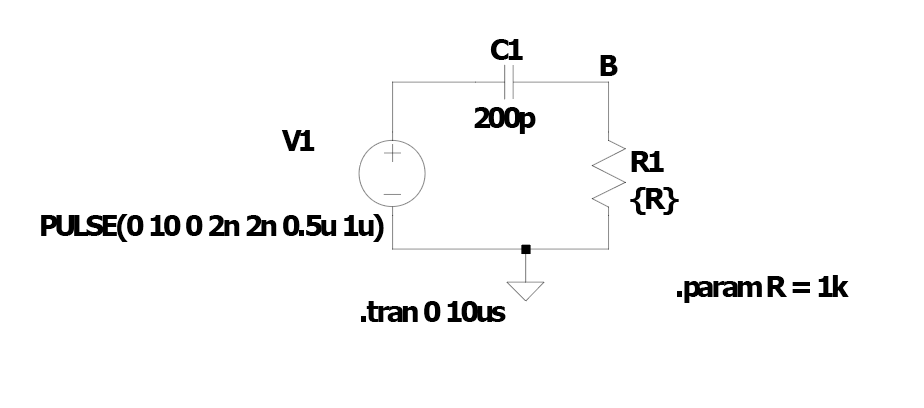
\includegraphics[width=\linewidth]{3aobwod}
		\caption{Schemat obwodu jednooczkowego dla symulacji czasowej parametrycznej.}
		\label{fig:3aobwod}
	\end{figure}
	
	Polecenie \texttt{.tran 0 10us} inicjuje symulację czasową, która trwa \(10 \mu s\). Dyrektywa \texttt{.param R=1k} ustawia wartość rezystancji \(R1\) na \(1 k\Omega\). Przebieg czasowy napięcia wejściowego oraz spadek napięcia na kondensatorze będzie prezentowany na wykresie.
	
	\begin{figure}[H]
		\centering
		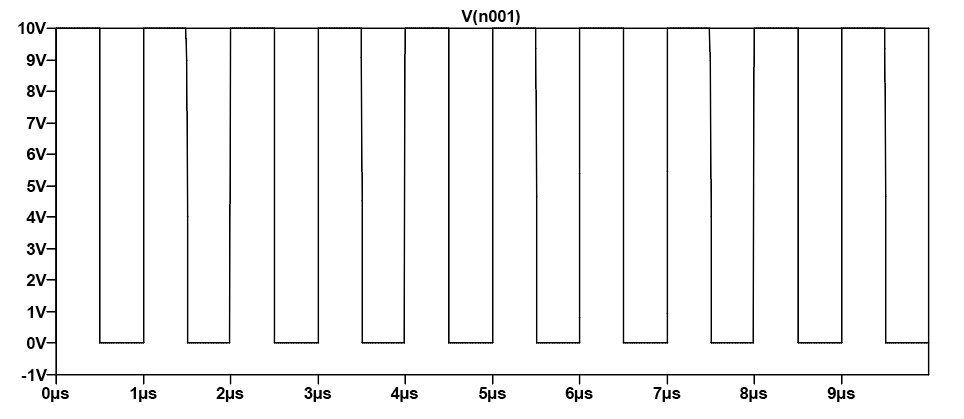
\includegraphics[width=\linewidth]{3awykres.png}
		\caption{Przebieg napięcia wejściowego oraz spadek napięcia na kondensatorze \(C1\) i napięcie na rezystorze \(R1\) w punkcie B.}
		\label{fig:3awykres}
	\end{figure}
	
	
	\pagebreak
	\subsection*{Podpunkt b}
	Dokonano symulacji czasowej dla obwodu zawierającego źródło napięcia V1, kondensator C1 oraz rezystor R1, aby zaobserwować dynamikę napięcia oraz prądu w odpowiedzi na sygnał prostokątny. Symulacja przeprowadzona została z rozdzielczością 1ns, aby szczegółowo obserwować zachowanie układu w krótkich przedziałach czasu.
	
	\begin{figure}[H]
		\centering
		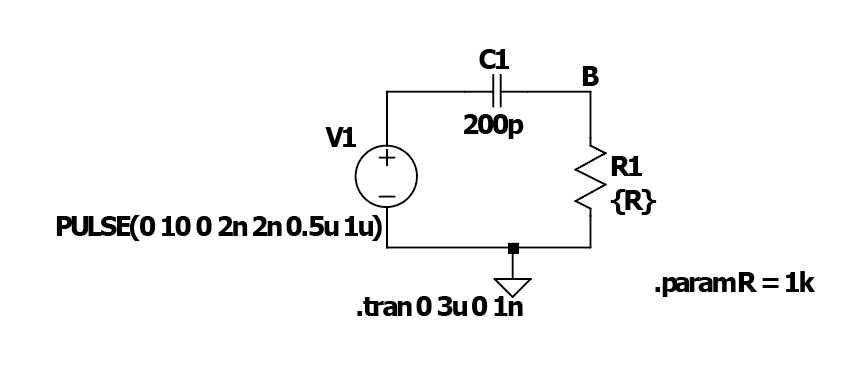
\includegraphics[width=0.8\linewidth]{3bobwod}
		\caption{Schemat obwodu wykorzystanego do symulacji czasowej z źródłem napięcia V1, kondensatorem C1 i rezystorem R1.}
		\label{fig:3bobwod}
	\end{figure}
	
	Na górnym panelu wykresu przedstawione jest napięcie wejściowe i na kondensatorze C1, natomiast dolny panel pokazuje napięcie na rezystorze R1 i prąd przez niego płynący. Wyniki te są zgodne z oczekiwaniami dla obwodu RC pod wpływem sygnału prostokątnego.
	
	\begin{figure}[H]
		\centering
		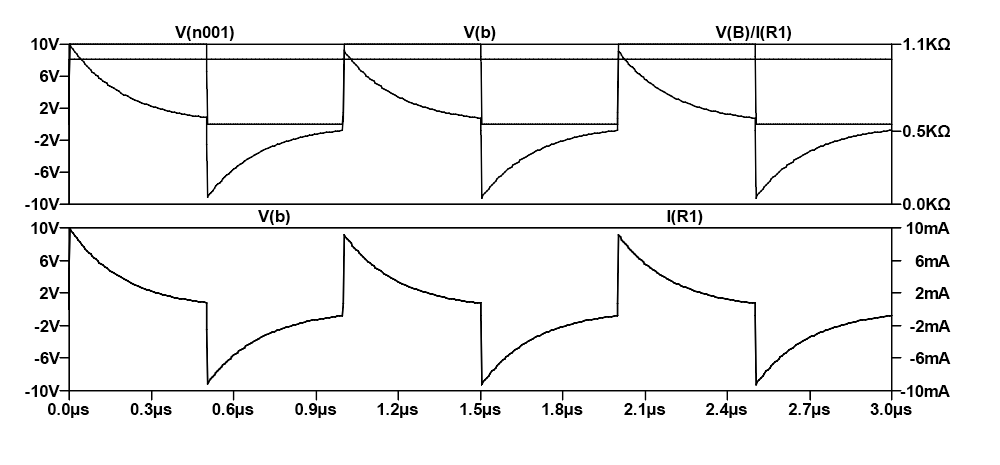
\includegraphics[width=\linewidth]{3bwykres}
		\caption{Na górnym panelu wykresu przedstawione jest napięcie wejściowe i na kondensatorze C1, natomiast dolny panel pokazuje napięcie na rezystorze R1 i prąd przez niego płynący.}
		\label{fig:3bwykres}
	\end{figure}
	
	W symulacji zaobserwowano, że stosunek napięcia na rezystorze do prądu płynącego przez niego jest stały, co jest zgodne z oczekiwaniami dla tego układu przy zadanych parametrach symulacji.


	
	\pagebreak
	\subsection*{Podpunkt c}
	W ramach analizy parametrycznej przeprowadzono serię symulacji czasowych, w których rezystancja R1 w obwodzie była zmienna. Ustawienia symulacji parametrycznej zdefiniowano przy użyciu dyrektywy \texttt{.step}, aby zmienność parametru R obejmowała zakres od 10 Ohm do 2 kOhm z dziesięcioma punktami na każdą dekadę wartości rezystancji.
	
	\begin{figure}[H]
		\centering
		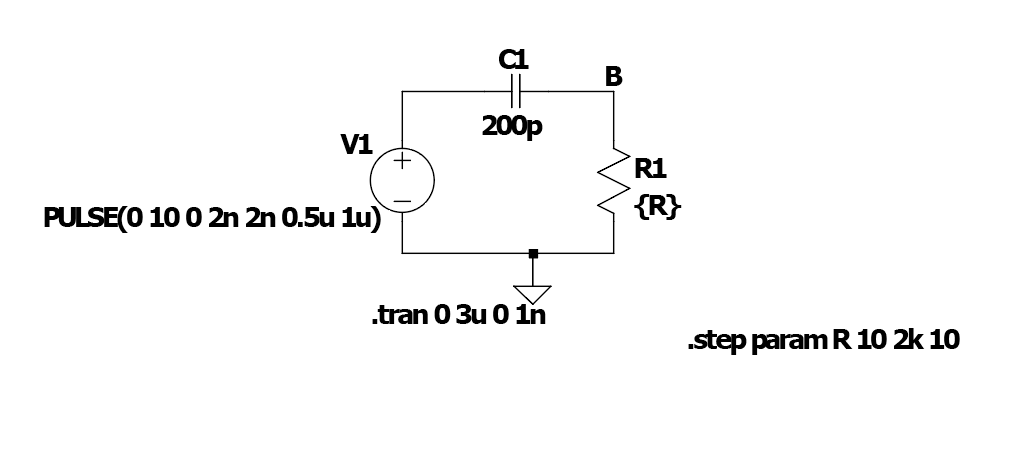
\includegraphics[width=0.8\linewidth]{3cobwod}
		\caption{Schemat obwodu wykorzystany w symulacji parametrycznej z źródłem V1, kondensatorem C1 i rezystorem R1.}
		\label{fig:3cobwod}
	\end{figure}
	
	\begin{figure}[H]
		\centering
		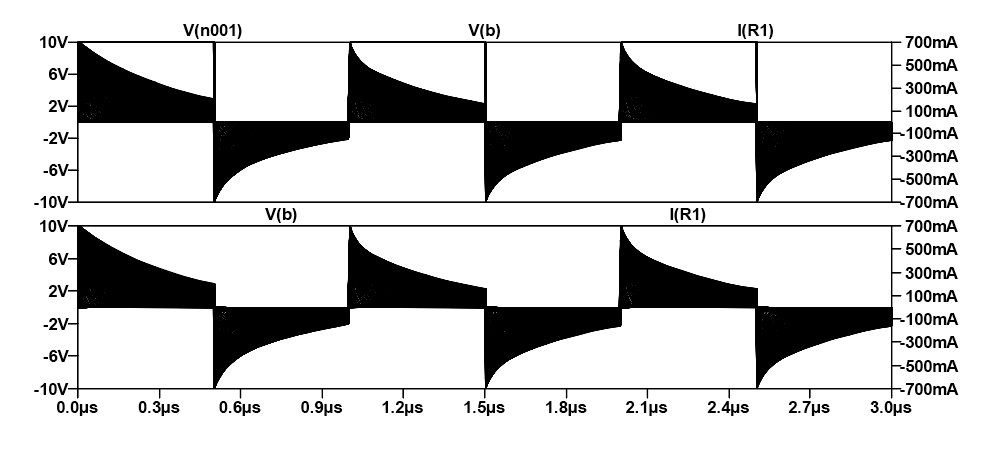
\includegraphics[width=\linewidth]{3cwykres}
		\caption{Seria wykresów przedstawiających prąd płynący przez rezystor R1 dla różnych wartości rezystancji w zadanej symulacji parametrycznej.}
		\label{fig:3cwykres}
	\end{figure}
	
	Zaobserwowano, że kształt prądu płynącego przez R1 zmienia się wraz z wartością rezystancji. Dla niższych wartości rezystancji, reakcja obwodu na zmiany sygnału jest szybsza, co prowadzi do większych szczytowych wartości prądu. Dla wyższych wartości R1, prąd przez rezystor ma mniejszą amplitudę, co jest zgodne z prawem Ohma, mówiącym, że prąd jest odwrotnie proporcjonalny do rezystancji w obwodzie przy stałym napięciu.
	
	Wykresy te demonstrują dynamiczną odpowiedź obwodu RC, która jest bezpośrednio związana z czasem ładowania i rozładowywania kondensatora C1. Wartości szczytowe prądu dla niższych rezystancji są wynikiem mniejszego oporu, który pozwala na szybszy przepływ prądu podczas ładowania i rozładowywania kondensatora. W miarę wzrostu rezystancji R1, czas reakcji obwodu wydłuża się, a prąd szczytowy maleje, co pokazuje dolny panel wykresu.
	
	Dane symulacji i ustawienia parametryczne potwierdzają zrozumienie charakterystyk obwodu RC i wpływ zmiennej rezystancji na zachowanie obwodu w czasie.
	
	\pagebreak
	\subsection*{Podpunkt d}
	Częstotliwość źródła napięcia $V1$ została zmieniona na wartość określoną przez wzór $160268*10$ Hz, zachowując 50\% wypełnienie przebiegu. W celu zidentyfikowania rezystancji $R1$, przy której napięcie na kondensatorze $C1$ osiąga 90\% wartości $V1$ w czasie równym 1/10 okresu przebiegu wejściowego, przeprowadzono symulację parametryczną.
	
	\begin{figure}[H]
		\centering
		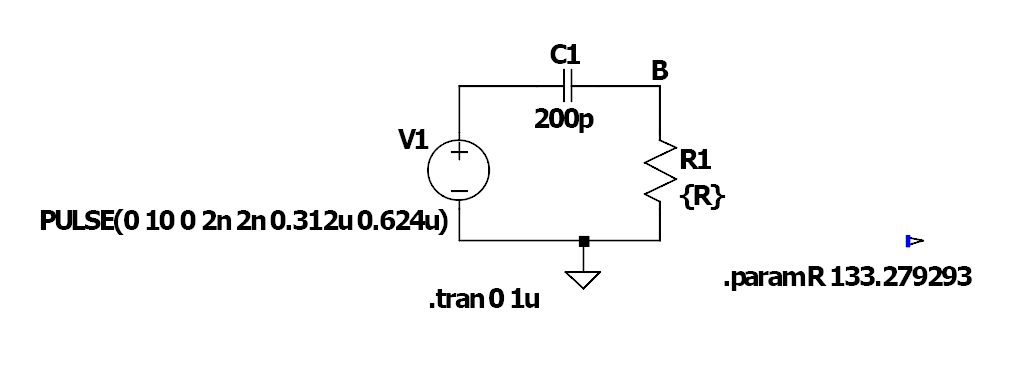
\includegraphics[width=0.8\linewidth]{3dobwod}
		\caption{Schemat obwodu RLC użyty w symulacji z rezystancją $R1$ ustawioną na $133.279293 \Omega$ oraz źródłem $V1$ o zmienionej częstotliwości.}
		\label{fig:3dobwod}
	\end{figure}
	
	Symulacja ujawniła, że przy rezystancji $R1 = 133.279293 \Omega$, napięcie na kondensatorze $C1$ szybko osiągnęło 90\% wartości napięcia źródłowego $V1$, co potwierdza wpływ rezystancji na szybkość ładowania kondensatora w obwodzie.
	
	\begin{figure}[H]
		\centering
		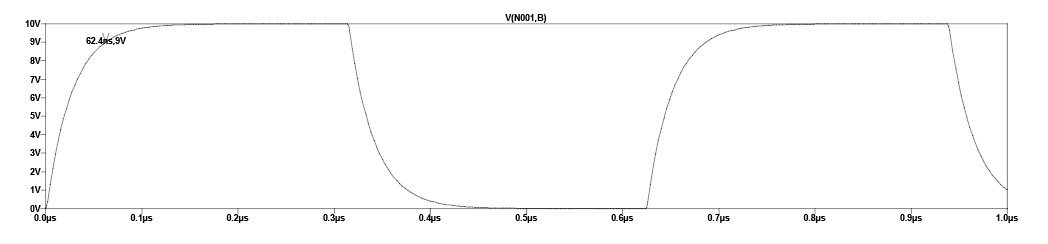
\includegraphics[width=\linewidth]{3dwykres}
		\caption{Wykres z symulacji ukazujący moment, w którym napięcie na kondensatorze $C1$ osiąga 90\% wartości źródła $V1$ przy rezystancji $R1 = 133.279293 \Omega$.}
		\label{fig:3dwykres}
	\end{figure}
	
	Szczegółowe dane z symulacji dla zmiennych wartości rezystancji są przedstawione w logu symulacji, gdzie analiza czasu ładowania kondensatora została przeprowadzona dla każdej wartości rezystancji w cyklu.
	
	\begin{figure}[H]
		\centering
		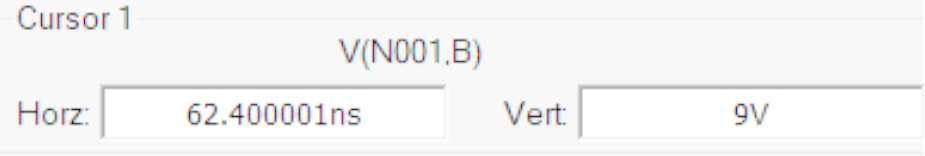
\includegraphics[width=\linewidth]{3dlog}
		\caption{Log symulacji przedstawiający wyniki pomiarów dla zmienionej częstotliwości źródła $V1$.}
		\label{fig:3dlog}
	\end{figure}
	
	\section*{Wnioski}
	Przeprowadzone eksperymenty pokazały, jak różne parametry wpływają na działanie obwodu. 
	
	
	
\end{document}
